\subsubsection{Backgrounds from particle misidentification}
\label{sec:backgrounds:misid}

A possible source of contamination comes from particles which are incorrectly identified as the
$\Kstarz\mumu$ final state.
A meson that decays via $\decay{X}{hh^\prime}$ which is then reconstructed
under the incorrect mass hypothesis could pass the selection criteria.
This type of contamination is studied by assigning different mass hypotheses to each final state
particle and calculating the invariant mass of the \mumu and \kpi candidates.
If the mass of one of these objects is seen to peak at the mass of a known particle, then the
contamination is removed  by applying \pid criteria to particles whose reassigned invariant mass
falls near $\mass{X}$.

Since a selection has been made on the \decay{\Kstarz}{\kpi} candidate using both \pid criteria and
constraints on the \kpi invariant mass it is expected that there will be little contamination
from background sources.
In order to be sure, \Kstarz candidates which come from a \Bd candidate which has an invariant mass
within $80\mev$ of the known \Bd mass are given different mass hypotheses to check for peaking
components in the new $\mass{K_{h}^+\pi_{h^\prime}^-}$ mass spectrum\footnote{
  Where, as defined previously, the notation $h_i$ is a particle under the mass hypothesis of $h$
  which was reconstructed as an $i$.
}.
The only background that must be removed from this category is from a real \decay{\phi}{\kk}
where a kaon in the final state is misidentified as being a pion.
If the mass of the $\Kp K^-_\pi$ candidate lies within $10\mev$ of the known \phii mass, the
ambiguous pion is subject to the requirements that
$\mathtt{ProbNNpi}<0.3$ and $\mathtt{ProbNNK>0.3}$.

Backgrounds from resonsaces decaying into a pair of hadrons which are then mistaken as a pair of
hadrons are more problematic.
Misidentification of the decay \decay{\KS}{\pipi} is already dealt with in the preslection, but
there is also contmaination from other long-lived hadronic states, namely the \Dz and \Lz.
The decays \decay{\Dz}{\kpi} and \decay{\Lz}{p\pim} are dealt with in a simiar way to the vetoes
described in \Sec{sec:dsphi:sel:veto}.
If the invariant mass of the $K^+_\mu\pi^-_\mu(p_\mu\pi^-_\mu)$ candidate falls within $25(10)\mev$
of the nominal $\Dz(\Lz)$ mass, then the ambiguous muon is subject to the requirement that
$\mathtt{ProbNNmu}>0.3(\mathtt{ProbNNp<0.3})$.


\begin{table}
  \caption{
   Vetoes from double and single misidentification of particles.
   If, under the alternate hypothesis, the \db or \Kstarz candidate mass falls within the range
   indicated under, the candidates are subject to the given \pid requirements.
  }
  \label{tab:bkg:vetoes}
  \begin{center}
    \begin{tabular}{lcc}\toprule
      \multicolumn{2}{c}{Mass criteria (MeV)} & PID requirement \\\midrule
      $\left|m(\Kp K^-_\pi) - m^\mathrm{PDG}_\phi\right|$ & $<10$
      & $\mathtt{ProbNNpi}(\pi)>0.3$ and {\tt ProbNNK$(\pi)<0.3$}
      \\\rule{0pt}{3ex}$\left|m(K^+_\mu\pi^-_\mu) - m^\mathrm{PDG}_{\Dz}\right|$& $<25$
      & $\mathtt{ProbNNmu}(\mu)>0.3$
      \\\rule{0pt}{3ex}$\left|m(p_\mu\pi^-_\mu) - m^\mathrm{PDG}_{\Lz}\right|$ & $<10$
      & $\mathtt{ProbNNp}(\mu)<0.3$  \\
      \bottomrule
    \end{tabular}
  \end{center}
\end{table}

There are also contributions from the decay \decay{\Bd}{\jpsi\Kstarz} and \decay{\jpsi}{\mumu},
where one of the hadron is misidentified as a muon, and vice versa.
This can be trivially removed by requiring that the hadrons do not satisfy {\tt isMuon}, as shown
in \Fig{fig:bkg:doublemisid}.

%\begin{figure}
  %\begin{center}
    %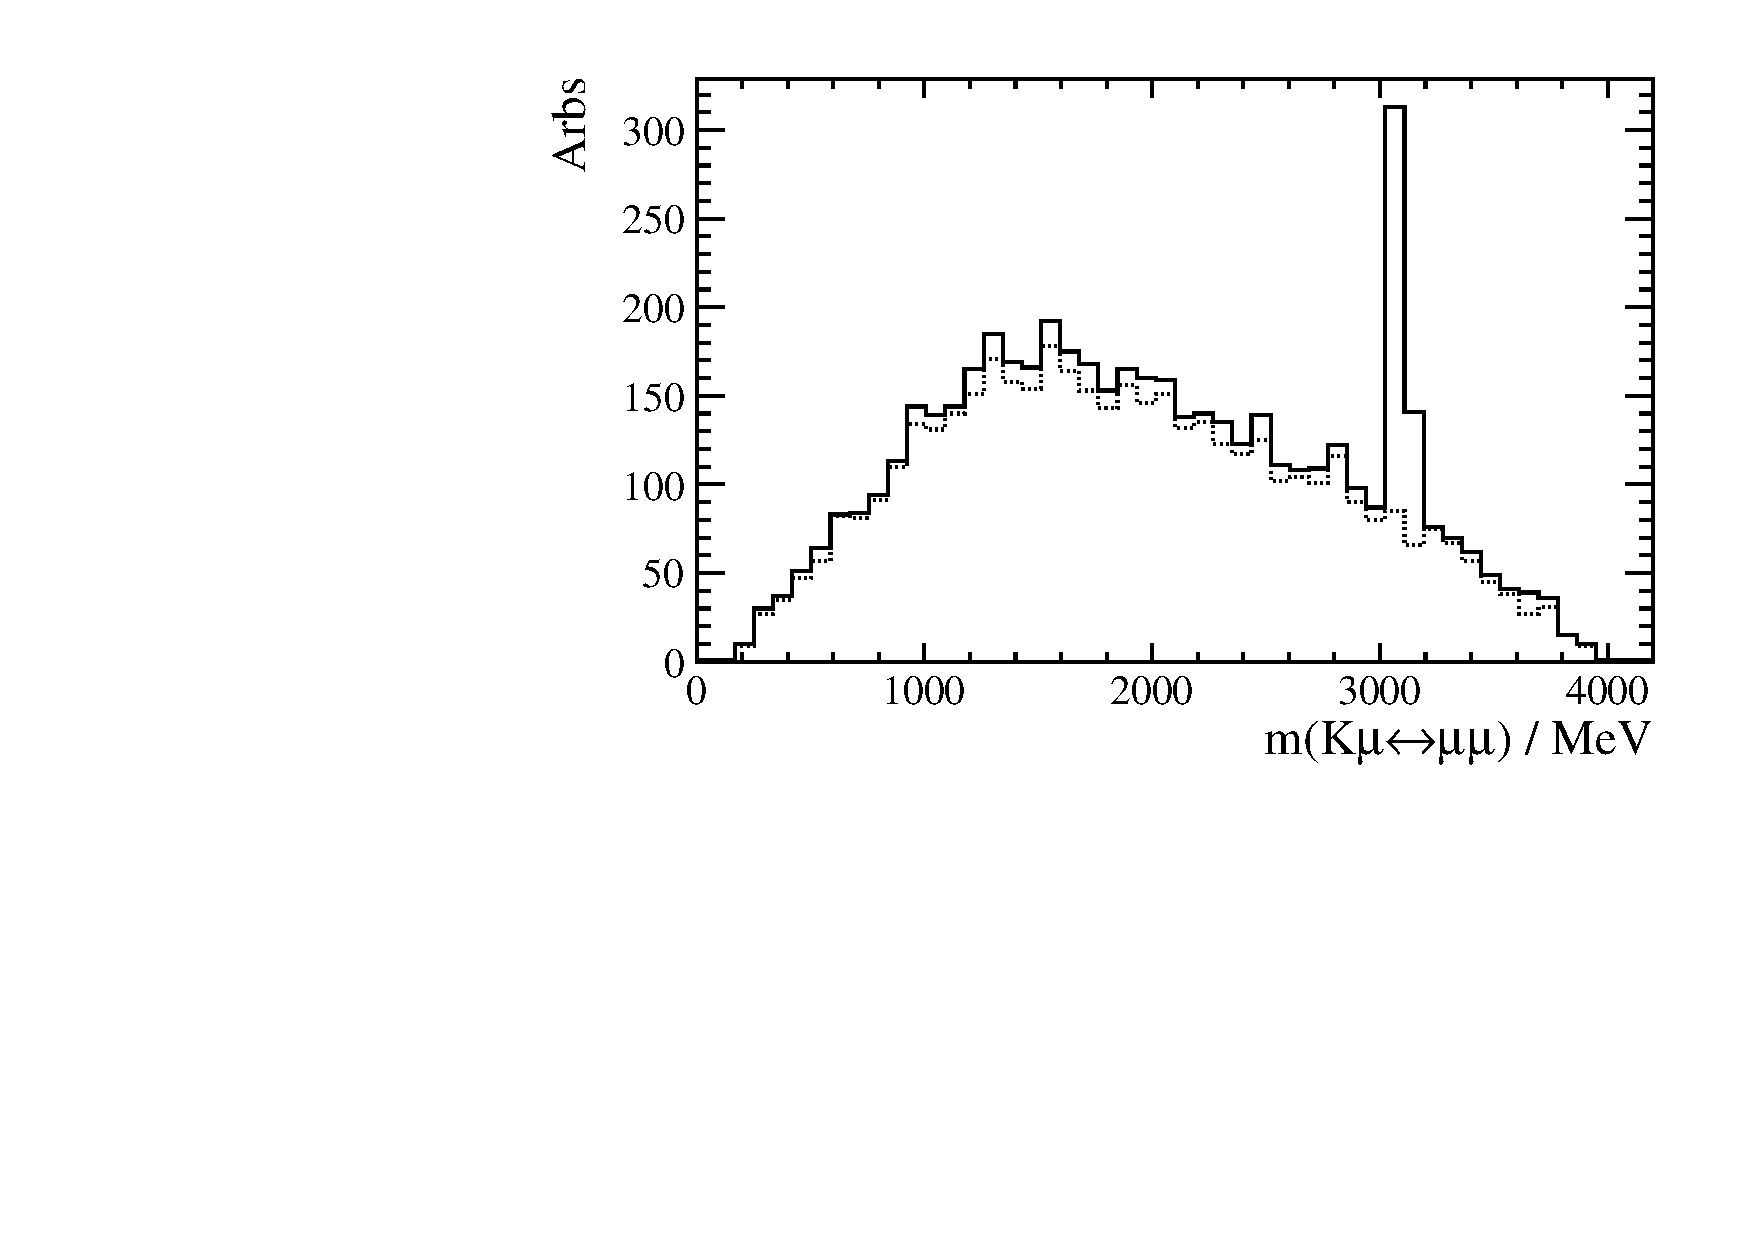
\includegraphics[width=0.48\textwidth]{double_misid_pi}
    %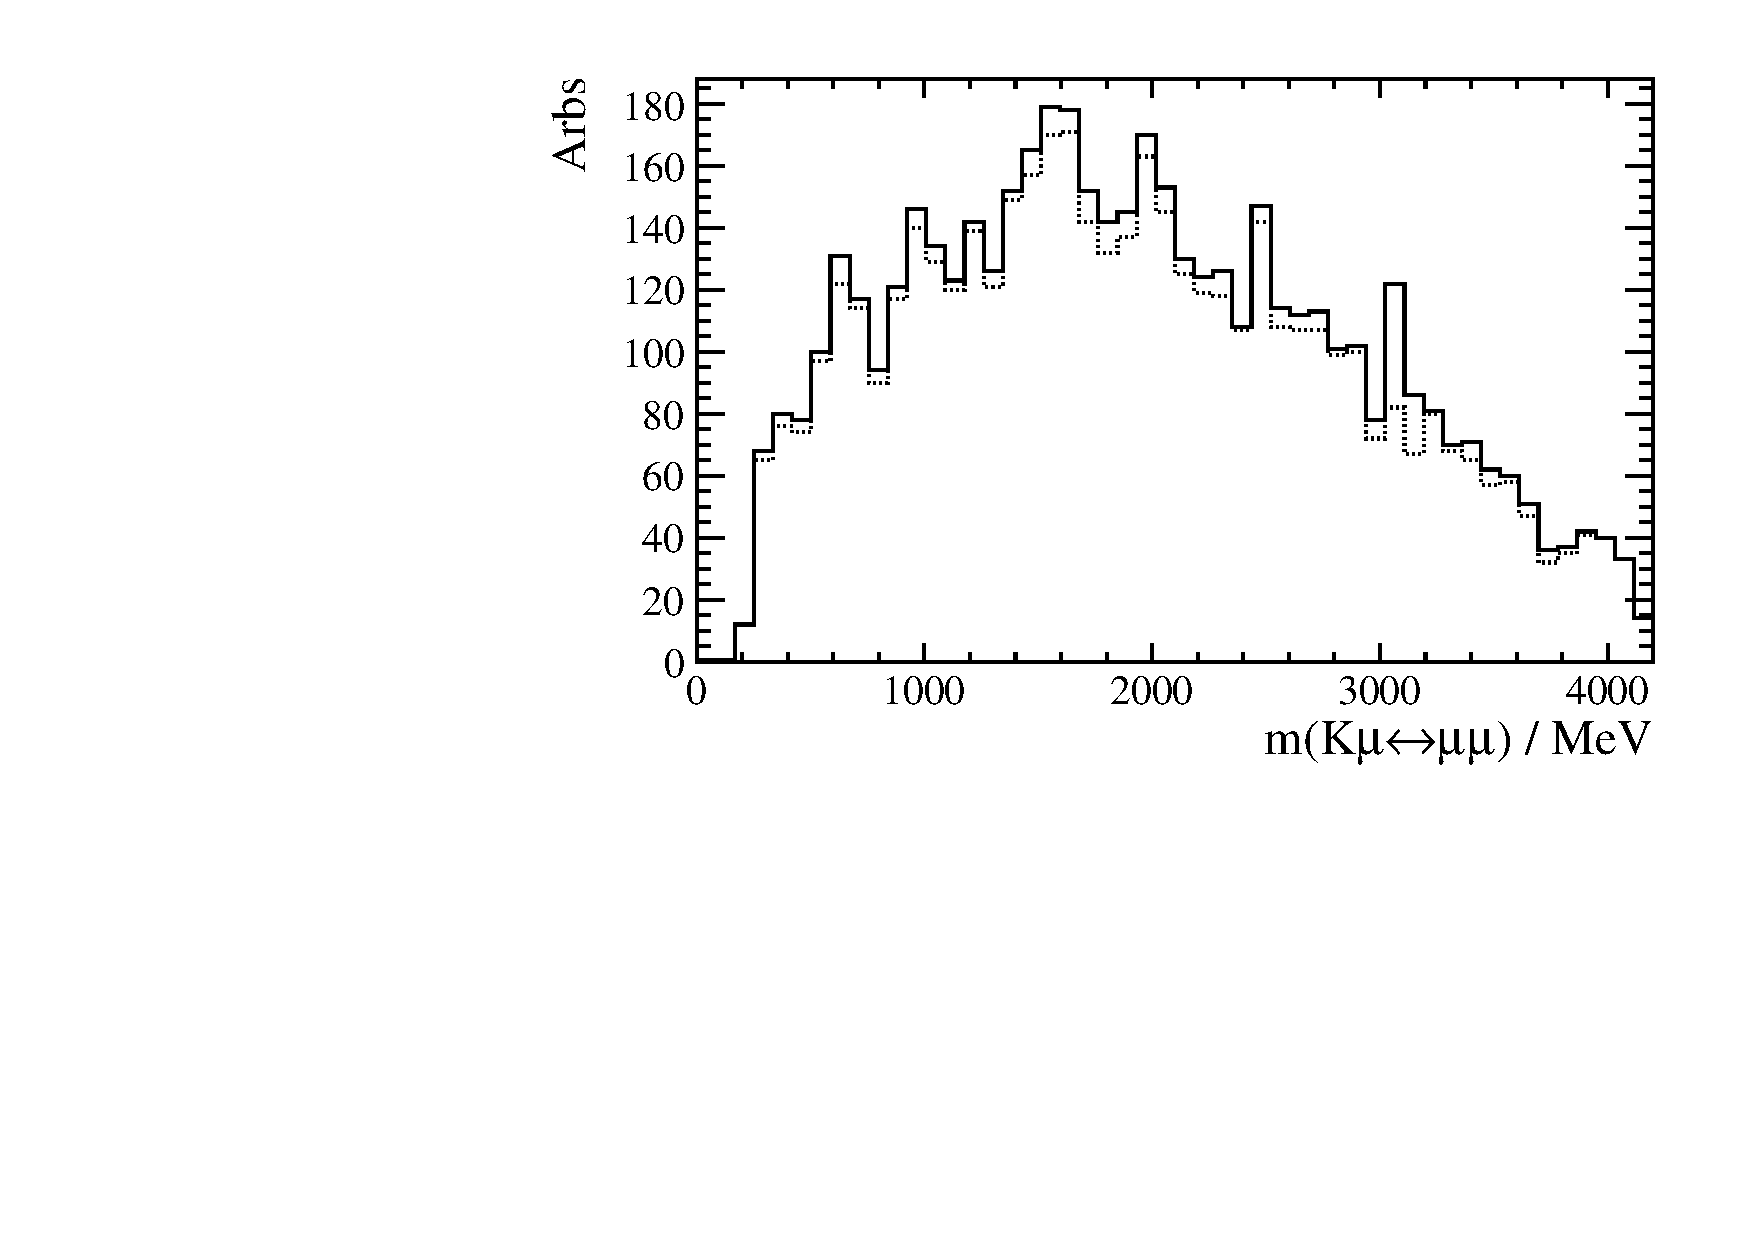
\includegraphics[width=0.48\textwidth]{double_misid_k}
    %\caption{\small
      %Background contributions from \decay{\Bd}{\jpsi\Kstarz}, where both a muon and (left) pion
      %and (right) kaon are misidentified as one another.
      %This background is very effectively removed by requiring that the hadron does not satisfy the
      %{\tt isMuon} criteria; the effect of this veto is shown with a dotted line.
    %}
    %\label{fig:bkg:doublemisid}
  %\end{center}
%\end{figure}

The sidebands are used to estimate the level of background in the signal region, and therefore
background
contributions are only problematic if they produce a narrow peaking structure in the dimuon mass.
Since misidentification results in smearing out of the mass, in general misidentification can only
cause a problem if the decaying particle has a very narrow natural width.
Therefore, any remaining misidentification-type backgrounds have negligible effect in the analysis.






